\documentclass[dvipsnames,table]{beamer}
\usepackage{polski}

\usetheme{Rochester}
\usecolortheme{orchid}

\usepackage{listings}
\usepackage{ucs}
\usepackage[utf8x]{inputenc}
\usepackage{wasysym}
\usepackage[normalem]{ulem}
\usepackage{amsmath}
\usepackage{hyperref}
\usepackage{tikzsymbols}

\setbeamertemplate{navigation symbols}{}
\setbeamertemplate{caption}[numbered]
\setbeamerfont{caption}{size=\scriptsize}
\setbeamercolor{framenote}{bg=OSEC-red!25}
\setbeamercolor{rednote}{bg=Red!25}
\setbeamercolor{palette primary}{use=structure,fg=white,bg=OSEC-red}
\setbeamercolor{palette secondary}{use=structure,fg=white,bg=OSEC-red2}

\setbeamertemplate{itemize item}{\scriptsize\raise1pt\hbox{\donotcoloroutermaths$\blacktriangleright$}}
\setbeamertemplate{itemize subitem}{\tiny\raise1pt\hbox{\donotcoloroutermaths$\bullet$}}
\setbeamertemplate{itemize subsubitem}{\tiny\raise1pt\hbox{\donotcoloroutermaths{--}}}

\setbeamertemplate{enumerate item}{\insertenumlabel.}
\setbeamertemplate{enumerate subitem}{\insertenumlabel.\insertsubenumlabel}
\setbeamertemplate{enumerate subsubitem}{\insertenumlabel.\insertsubenumlabel.\insertsubsubenumlabel}
\setbeamertemplate{enumerate mini template}{\insertenumlabel}

\setbeamercolor{itemize item}{fg=OSEC-red, bg=OSEC-red}
\setbeamercolor{itemize subitem}{fg=OSEC-red, bg=OSEC-red}
\setbeamercolor{itemize subsubitem}{fg=OSEC-red, bg=OSEC-red}

\setbeamercolor{section number projected}{fg=white,bg=OSEC-red}
\setbeamercolor{subsection number projected}{fg=white,bg=OSEC-red}
\setbeamercolor{button}{bg=OSEC-red,fg=white}

\setbeamertemplate{section in toc}[circle]
\setbeamertemplate{subsection in toc}[square]

\definecolor{OSEC-red}{RGB}{160,29,44}
\definecolor{OSEC-red2}{RGB}{177,76,12}
\hypersetup{colorlinks=true,linkcolor=white,urlcolor=OSEC-red}

\setlength{\tabcolsep}{8pt}
\renewcommand{\arraystretch}{1.2}

\newcommand{\tri}{$\triangleright$ }

\lstset{
   language=C,
   basicstyle=\tiny,
   breaklines=true,
   escapechar=\@,
}

\title{Gdy CPU nie wystarcza –- strategie optymalizacji oprogramowania z użyciem technologii GPU oraz FPGA}
\author{Radosław Kujawa -- radoslaw.kujawa@osec.pl}
\institute{OSEC}

\begin{document}

\begin{frame}
	\titlepage
\end{frame}

\begin{frame}
	\frametitle{Dlaczego GPU i FPGA do obliczeń?}
\begin{itemize}
	\item Wydajność procesorów nie rośnie już tak szybko\dots
	\item Ograniczona wydajność pojedyńczego rdzenia procesora.
	\item Procesory: mała ilość skomplikowanych jednostek ALU.
	\item Do przyśpieszenia obliczeń (wykorzystania wielu rdzeni) i tak musimy je zrównoleglić.
	\item GPGPU -- General Purpose computing on a Graphics Processing Unit. 
	\item Układy GPU: {\em bardzo} duża ilość prostych jednostek ALU, bardzo wysoka wydajność pamięci.
	\item FPGA -- Field Programmable Gate Array.
	\item Układy FPGA: Możliwość konfiguracji bramek logicznych na poziomie sprzętowym, do zaimplementowania konkretnego algorytmu.
	
\end{itemize}
\end{frame}

% krótki wstęp do arch. GPU i FPGA

\begin{frame}
	\frametitle{Obszary zastosowań GPGPU oraz FPGA} 
\begin{itemize}
	\item Badania naukowe wymagające skomplikowanych obliczeń matematycznych.
	\begin{itemize}
		\item Chemia.
		\item Biologia.
		\item Fizyka.
	\end{itemize}
	\item Akceleracja obliczeń w grach i multimediach.
	\item Akceleracja przeglądarek:
	\begin{itemize}
		\item Chrome.
		\item Firefox.
	\end{itemize}
	\item Modele probabilistyczne.
	\item Kryptografia.
	\begin{itemize}
		\item Szyforwanie.
		\item Funkcje skrótu.
	\end{itemize}
	\item Wydobycie walut kryptograficznych.
\end{itemize}
\end{frame}

\begin{frame}
	\frametitle{Nvidia CUDA}
\begin{itemize}
	\item Dobra wydajność i optymalizacja pod kątem GPU Nvidia.
	\item Closed source.
	\item Vendor lock-in.
	\item Gotowe biblioteki BLAS, FFTW, NPP, itd.
	\item Słaba integracja z dystrybucjami Linuxa.
	\item Dobre materiały edukacyjne.
	\item Duża popularność w środowisku akademickim.
	\item Kod C kompilowany kompilatorem C++. \Annoey
\end{itemize}
\begin{center}
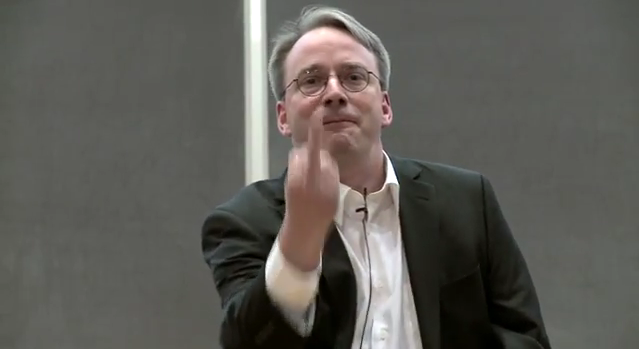
\includegraphics[scale=0.25]{img-torvalds.png}

\includegraphics[scale=0.19]{img-stallman.jpg}
\end{center}


\end{frame}

\begin{frame}
	\frametitle{OpenCL}
\begin{itemize}
	\item Otwarty standard grupy Khronos.
	\item Jak OpenGL\ldots tylko do obliczeń.
	\item Analogiczna infrastruktura oparta o ,,Installable Client Driver'', dostarczany przez dostawcę sprzętu (lub systemu operacyjnego).
	\item Idea podobna do CUDA -- tworzymy specjalny, dedykowany kod wykonujący się na koprocesorze (,,kernel'').
	\item API do obliczeń nie tylko na GPU, lecz też CPU, FPGA\ldots
	\item Najnowsza wersja standardu 2.2, ale dostawcy powolni w implementacji (NVidia - 1.2, Mesa Clover 1.1).
\end{itemize}
\end{frame}


\begin{frame}[fragile]
	\frametitle{Implementacje OpenCL}
\begin{table}[]
\centering
\caption{Najpopularniejsze implementacje OpenCL.}
\label{porownanie}
\scriptsize
\begin{tabular}{llll}
\hline
Implementacja &  Urządzenia  & Open source   \\ \hline
Apple OpenCL & GPU AMD/Nvidia/Intel & Nie \\
AMDGPU Pro & GPU AMD & Nie \\
Beignet & GPU Intel & Tak \\
Intel FPGA SDK for OpenCL & FPGA Altera & Nie \\
Intel Graphics Compute Runtime & GPU Intel Gen8+ & Tak \\
pocl & CPU, GPU (CUDA) & Tak \\
ROcm & GPU AMD i CPU & Tak \\
Nvidia OpenCL & GPU Nvidia & Nie \\
Mesa Clover & GPU AMD/Nvidia & Tak \\
Xilinx SDAccel & FPGA Xilinx & Nie \\ \hline
\end{tabular}
\normalsize
\end{table}
\end{frame}

\begin{frame}
	\frametitle{Algorytmy a wykonanie na GPU/FPGA}
\begin{itemize}
	\item Od początku istnienia komputerów, większość algorytmów była projektowana jako algrytmy sekwencyjne.
	\item GPU i FPGA wymagają algorytmów równoległych aby efektywnie wykorzystać możliwości sprzętu.
	\item Konwersja algorytmu w równoległy: wyodrębnienie części algorytmu, która może wykonywać się równolegle.
	\item Nie każdy algorytm da się zrównoleglić.
	\item \href{http://www.mcs.anl.gov/~itf/dbpp/text/book.html}{Ian Foster -- Designing and Building Parallel Programs}
	\begin{itemize}
		\item Partitioning -- find possible ways to split the data among the workers as fine-grain as possible.
		\item Communication -- identify the communication patterns.
		\item Agglomeration -- reduce the initial partitions to coarse-grain tasks according to the resources available.
		\item Mapping -- map the tasks onto the processing units.
	\end{itemize}
%	\item \href{http://legacydirs.umiacs.umd.edu/~vishkin/PUBLICATIONS/classnotes.pdf}{Uzi Vishkin -- Thinking in Parallel: Some Basic Data-Parallel Algorithms and Techniques}
\end{itemize}
\end{frame}

%\begin{frame}
%\frametitle{foo}
%\includegraphics[width=1.00\textwidth]{img-bar.pdf}
%\end{frame}

\begin{frame}
	\frametitle{CUDA i OpenCL -- wspólne wady}
\begin{itemize}

	\item Niskopoziomowe programowanie równoległe jest trudne.
	\item Możliwe rozwiązania: 
	\begin{itemize}
	\item Użycie języków programowania wyższego poziomu do implementacji algorytmów - np. PyCUDA\ldots
	\item Użycie mechanizmów ułatwiających pisanie programów na GPU/FPGA w C/C++ - np. OpenACC.
	\item Użycie gotowych bibliotek dziedzinowych - np. BLAS.
	\end{itemize}
\end{itemize}
\begin{center}
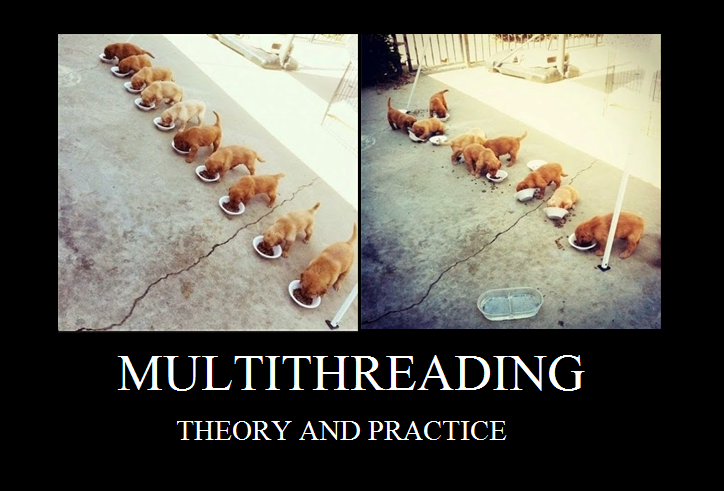
\includegraphics[scale=0.25]{img-threadpuppies.png}
\end{center}
\end{frame}

\begin{frame}
	\frametitle{OpenACC}
\begin{itemize}
	\item Deklaracje w zwykłym kodzie C/C++.
	\item Wysoki poziom, bez potrzeby pisania osobnego kodu dla GPU/FPGA.
	\item Backend open source generujący kod nvptx (CUDA).
	\item Niedługo wsparcie dla AMD (\href{https://gcc.gnu.org/ml/gcc/2018-05/msg00071.html}{port Mentor Graphics}).
	\item \href{https://www.psc.edu/images/xsedetraining/OpenACC_Mar2016/OpenACC_Introduction_To_OpenACC.PDF}{John Urbanic -- Introduction to OpenACC}
\end{itemize}
\end{frame}



\begin{frame}[fragile]
	\frametitle{Przykład: OpenACC}
\begin{lstlisting}
/* gcc src.c -fopenacc -foffload=nvptx-none -foffload="-O3" -O3 -o exec */
#include <stdio.h>
#define N 2000000000

int main(void) {
	double pi = 0.0f;
	long long i;

	#pragma acc parallel
	#pragma acc loop reduction(+:pi)
	for (i = 0; i < N; i++) {
		double t = (double)((i+0.5)/N);
		pi +=4.0/(1.0+t*t);
	}

	printf("pi=%11.10f\n",pi/N);

	return 0;
}
\end{lstlisting}
\end{frame}

\begin{frame}
	\frametitle{Biblioteki wyższego poziomu}
\begin{itemize}
	\item Przyśpieszenie "drop-in", bez potrzeby zgłębiania technik programowania równoległego, GPU, FPGA, itd.
	\item Łatwiejsze w obsłudze, niższy próg wejścia niż do CUDA/OpenCL.
	\item Wiele gotowych bibliotek dla specyficznych dziedzin programowania.
	\begin{itemize}
		\item OpenCV.
		\item Basic Linear Algebra Subprograms (BLAS).
		\item TensorFlow.
		\item \ldots 
	\end{itemize}
\end{itemize}
\end{frame}

\begin{frame}
	\frametitle{BLAS -- Basic Linear Algebra Subprograms} 
\begin{itemize}
	\item Przykład biblioteki wysokiego poziomu zoptymalizowanej dla GPU/FPGA.
	\item \href{http://www.netlib.org/blas/}{CBLAS (CPU)}.
	\item \href{https://docs.nvidia.com/cuda/cublas/index.html}{cuBLAS (CUDA)}.
	\item \href{https://github.com/CNugteren/CLBlast}{CLBlast (OpenCL)}.
	\item \href{https://developer.apple.com/documentation/accelerate/blas}{Accelerate.framework (CPU SIMD, macOS)}.
	\item \ldots
\end{itemize}
\end{frame}

\begin{frame}[fragile]
\frametitle{Przykład: Mnożenie macierzy za pomocą  BLAS}
\begin{itemize}
	\item Funkcja {\tt sgemm} (poj. prezycja) / {\tt dgemm} (podwójna precyzja).
\end{itemize}
\begin{lstlisting}
void cblas_sgemm(const CBLAS_LAYOUT layout, const CBLAS_TRANSPOSE TransA,
	const CBLAS_TRANSPOSE TransB, const int m, const int n,
	const int k, const float alpha, const float  *A,
	const int lda, const float  *B, const int ldb,
	const float beta, float  *C, const int ldc);
\end{lstlisting}
\[ C \leftarrow \alpha op(A) op(B) + \beta C \]
\begin{itemize}
	\item $op(X)$ to $op(X) = X$, lub $op(X) = X^T$ lub $op(X) = X^H$.
	\item $\alpha$ i $\beta$ są skalarami.
	\item $A$, $B$ i $C$ są macierzami.
	\item $op(A)$ jest macierzą $m$ x $k$.
	\item $op(B)$ jest macierzą $k$ x $n$.
	\item $C$ jest macierzą $m$ x $n$.
\end{itemize}
\end{frame}

\begin{frame}[fragile]
	\frametitle{Przykład: Mnożenie macierzy za pomocą BLAS c.d.}
\begin{itemize}
	\item Prawdopodobnie najprostszy możliwy przypadek -- mnożenie dwóch macierzy, o takich samych rozmiarach, bez dodatkowych operacji. 
	\item $A$ oraz $B$ mają rozmiar 1000 x 1000.
\end{itemize}
\scriptsize
\[
A =
\begin{bmatrix}
	a_{0} & a_{1} & \dots & a_{999} \\
	a_{1000} & a_{1001} & \dots & a_{1999} \\
	\dots & \dots & \dots & \dots \\
	a_{999000} & a_{999001} & \dots & a_{999999} \\
\end{bmatrix}
, B = 
\begin{bmatrix}
	b_{0} & b_{1} & \dots & b_{999} \\
	b_{1000} & b_{1001} & \dots & b_{1999} \\
	\dots & \dots & \dots & \dots \\
	b_{999000} & b_{999001} & \dots & b_{999999} \\
\end{bmatrix}
\]
\[
C = A \times B
\]
\normalsize
\begin{lstlisting}
cblas_sgemm(CblasRowMajor, CblasNoTrans, CblasNoTrans, 1000, 1000, 1000,
	1.0f, a, 1000, b, 1000, 1.0f, c, 1000);
\end{lstlisting}
\end{frame}

\begin{frame}
\frametitle{Benchmark - mnożenie macierzy 5000 x 5000}
\begin{table}[]
\centering
\caption{Porównanie czasów wykonania programu mnożącego macierz z użyciem funkcji sgemm.}
\label{porownanie}
\scriptsize
\begin{tabular}{llll}
\hline
Implementacja & CPU/GPU   & System operacyjny & Czas  \\ \hline
CBLAS 3.8.0   & AMD E-350 1.6GHz & Fedora 28         & 6m41s \\
% Accelerate.framework & Intel Core M-5Y51  & macOS 10.13 & 0m9s  \\
cuBLAS (CUDA 9.1) & GeForce GTX 1050 Ti & Fedora 28 & 0m5s  \\ \hline
\end{tabular}
\normalsize
\end{table}
\end{frame}

\begin{frame}
\frametitle{Więcej informacji...}
\begin{itemize}
	\item \href{https://www.x.org/wiki/Events/XDC2017/Stellard_GPGPU.pdf}{Tom Stellard -- Current State of Open Source GPGPU - XDC2017}
	\item \href{https://developer.nvidia.com/sites/default/files/akamai/cuda/files/Misc/mygpu.pdf}{Andrzej Chrzęszczyk, Jacob Anders -- Matrix computations on the GPU - CUBLAS, CUSOLVER and MAGMA by example}

\end{itemize}
\end{frame}

\begin{frame}
	\frametitle{GPGPU i FPGA w chmurze}
\begin{itemize}
	\item Amazon (GPU, FPGA)
	\begin{itemize}
		\item Amazon EC2 \href{https://aws.amazon.com/ec2/instance-types/f1/}{F1}.
		\item Amazon EC2 G3, P3, Elastic GPUs.
	\end{itemize}
	\item \href{https://cloud.google.com/gpu/}{Google Cloud (GPU)}
	\item \href{https://www.nimbix.net/xilinx/}{Nimbix (FPGA)}
\end{itemize}
\end{frame}

%\begin{frame}
%\frametitle{Przyszłość}
%	\begin{itemize}
%		\item OpenCL Next
%	\end{itemize}
%\end{frame}

\begin{frame}
\frametitle{Koniec\ldots}
\begin{center}

\includegraphics[scale=0.5]{img-oseclogo.png}

Dziękuje!

Czy są pytania?

\end{center}
\end{frame}
\end{document}

